\chapter{El sitio}
\label{cap:sitio}

\section{Vistas}

El sitio (\href{https://cadlag.vercel.app}{cadlag.vercel.app}) es un Next.js exportado como HTML estático. No tiene servidor: todo lo que calcula, lo calcula el navegador con los archivos que se descargaron al compilar. Tiene cuatro tipos de páginas.

\begin{itemize}
\item \textbf{Inicio}: el resumen de cada liga y copa con su favorito y su probabilidad, la historia de una temporada contada con la trayectoria de su campeón (figura~\ref{fig:trayectoria}) y una explicación corta del modelo, de los resultados que funcionaron y de los que no.
\item \textbf{Liga}: la matriz de posiciones finales con las zonas de cada liga, columnas extra según el formato (ascenso, playoffs, campeón del torneo, descenso, copas del año siguiente), el laboratorio ``¿Y si…?'', los partidos decisivos y la ficha de cada equipo con sus fuerzas, la curva de ``qué necesita'' y sus cotas matemáticas.
\item \textbf{Copa}: para la Champions, la matriz de la fase liga con columnas de octavos, cuartos, semis, final y campeón; para la Libertadores y la Sudamericana, las llaves abiertas, la tabla de ``hasta dónde llega'' y los grupos, con su laboratorio durante la fase de grupos.
\item \textbf{Mundo}: la comparación entre ligas de la red del capítulo~\ref{cap:red}, con la fuerza neta de cada liga, el grafo de partidos y un ranking global de clubes en escala común.
\end{itemize}

\begin{figure}[h]
\centering
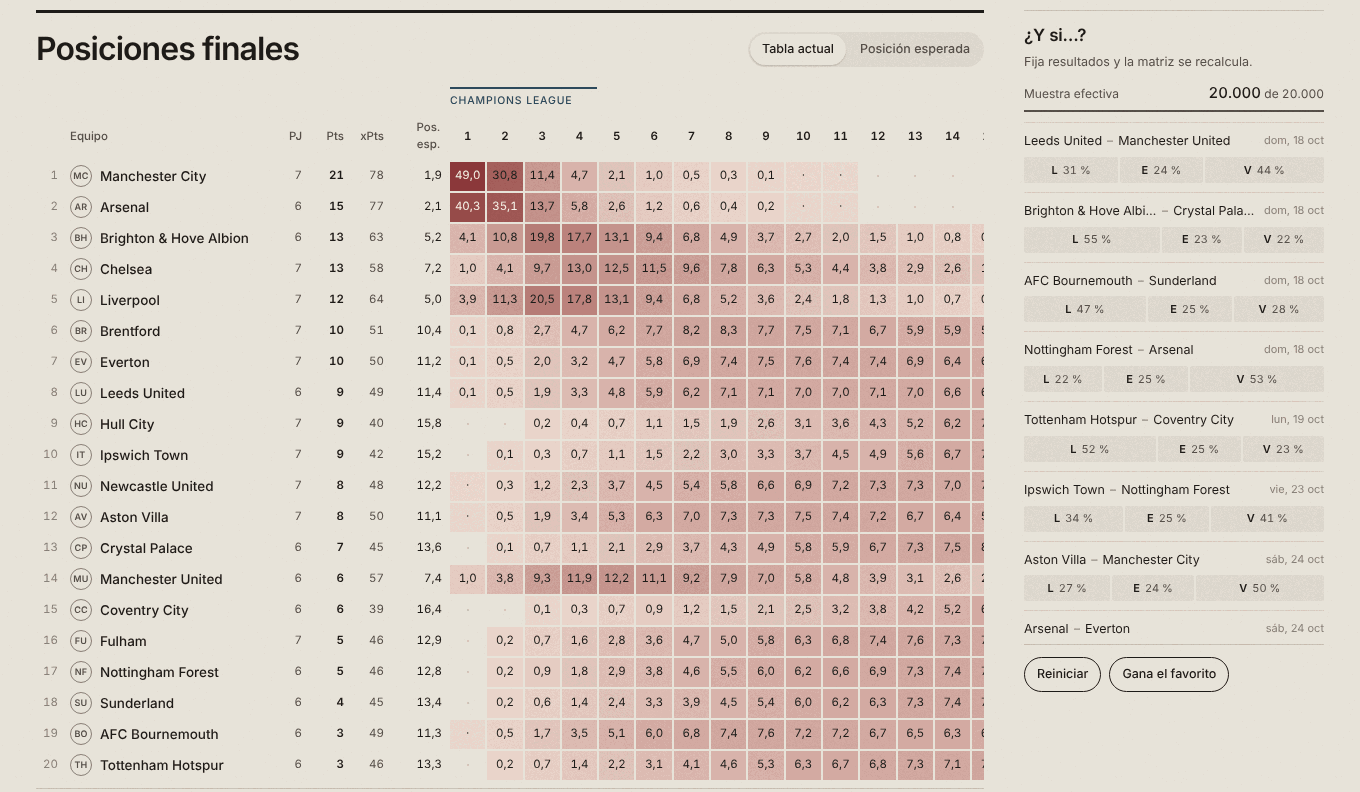
\includegraphics[width=\textwidth]{sitio_matriz}
\caption{La matriz de la Premier en el sitio, con el panel del laboratorio a la derecha. Las celdas usan una escala de calor que se recalcula con el tema claro u oscuro.}
\label{fig:sitio}
\end{figure}

\section{El laboratorio en el navegador}

Para cada liga se publica, junto al JSON del pronóstico, un archivo binario comprimido con las 20.000 temporadas simuladas, de unos 1,1 a 2,4 MB. Cada temporada ocupa un registro de $W$ bytes con el resultado sorteado de los próximos diez partidos, sus probabilidades dadas las fuerzas de esa temporada y, para cada equipo, sus puntos y su posición final (formato completo en el apéndice~\ref{ap:formato}).

Las probabilidades se guardan como $\lfloor255\sqrt p\rceil$ en un byte. La raíz da precisión relativa donde importa: una probabilidad de 0,01 se guarda con un error relativo de un 4\,\%, en vez del 40\,\% que tendría con una escala lineal, y al multiplicar varias en el peso $w_s$ los errores relativos se suman en vez de explotar. El navegador decodifica con una tabla de 256 entradas.

Al fijar un resultado, el navegador recorre las 20.000 temporadas: multiplica el peso, corrige los puntos de los dos equipos si el resultado sorteado era otro, reordena la tabla y acumula la matriz ponderada. Son unos 20.000 $\times$ 20 equipos operaciones por escenario, que en un \code{Float64Array} toman milisegundos. Lo que depende de una llave posterior a la tabla (el ascenso por playoffs, el campeón de un torneo argentino, las rondas de una copa) usa las tablas $P(\text{lo logra}\mid\text{equipo},\text{posición})$, que el navegador calcula una sola vez al cargar el archivo. Las probabilidades de los partidos que siguen abiertos también se recalculan: al fijar una derrota del favorito, sus próximos partidos se ven un poco menos favorables.

\begin{figure}[h]
\centering
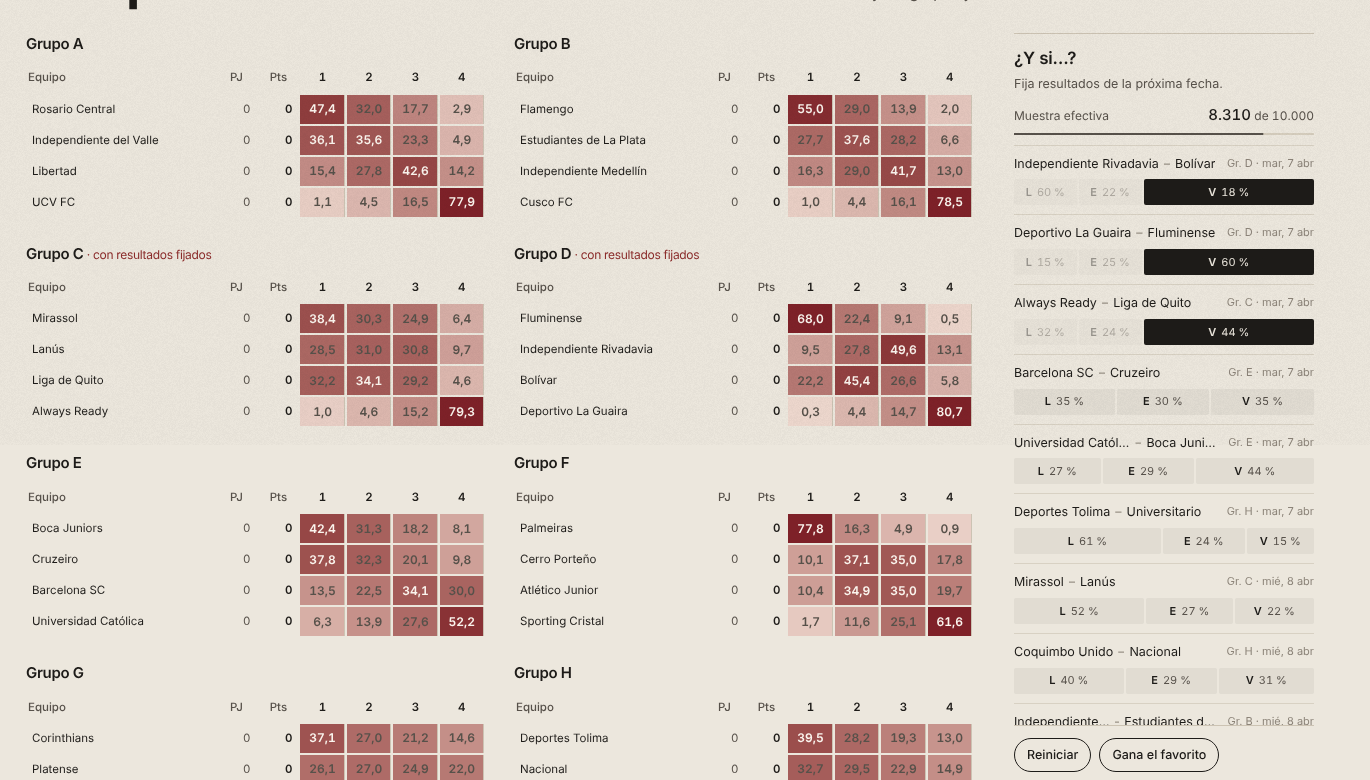
\includegraphics[width=\textwidth]{lab_libertadores}
\caption{El laboratorio de la fase de grupos de la Libertadores, probado con la edición 2026 vista antes de la primera fecha. Con tres resultados fijados (gana la visita en los tres primeros partidos) los grupos C y D se recalculan y la muestra efectiva baja a 8.310 de 10.000.}
\label{fig:lab}
\end{figure}

La figura~\ref{fig:lab} muestra el laboratorio de grupos de la capítulo~\ref{cap:escenarios}. Fijar que Liga de Quito gana en la altura de El Alto le sube en 14,3 puntos la probabilidad de llegar a octavos; fijar que Independiente Rivadavia pierde de local con Bolívar se la baja en 32,8, porque esa derrota también dice algo de su fuerza.

\section{Diseño}

La dirección visual es sobria: fondo de papel, una sola tinta, un solo color de acento (un rojo apagado) y una escala de calor para las probabilidades que respeta el orden perceptivo y funciona en tema claro y oscuro. Los números usan cifras tabulares, las probabilidades se muestran con un decimal y las menores a 0,05\,\% se dejan en blanco, para que la matriz se lea por sus manchas antes que por sus cifras. Todo el sitio está en español, con la convención de coma decimal.
